\chapter{Referencial Teórico}\label{sec:conceitos}
Neste capítulo são introduzidos os conceitos necessários para o entendimento deste trabalho e está organizado da seguinte forma. A Seção \ref{sec:recemo} define o que é o reconhecimento de emoção e os tipos de reconhecimento. A Seção \ref{sec:expfacia} fundamenta a expressão facial emocional e mostra as expressões básicas existentes. A Seção \ref{sec:apm} conceitua a área de aprendizagem de máquina. A Seção \ref{sec:pci} apresenta o processo de classificação de imagem. A Seção \ref{sec:tecnic} revisa as técnicas de pré-processamento que são utilizadas para eliminação de ruídos de uma imagem. As Seções \ref{sec:rna} e \ref{sec:rnc} conceituam os aspectos básicos das redes neurais artificiais e das redes neurais de convolução, respectivamente. A Seção \ref{sec:arc} descreve as arquiteturas de redes neurais de convolução utilizadas por este trabalho e para concluir a Seção \ref{sec:considf} faz um resumo acerca deste capítulo.   

\section{Reconhecimento de Emoção}\label{sec:recemo}
As emoções podem ser definidas como breves e intensas e são disparadas pela avaliação de um evento \citep{scherer2000psychological}. O reconhecimento de emoção tem sido explorado há algumas décadas e as emoções que tem sido frequentemente investigadas são as básicas como a raiva, alegria, tristeza, desgosto, medo e surpresa \citep{ekman1994}. Com objetivo de reconhecer emoção, os pesquisadores têm utilizado comumente as técnicas de reconhecimento de padrões, que por sua vez podem encontrar as características que são importantes para diferenciar as emoções, isto é, a busca pelo padrão relevante de uma entrada de dados, por exemplo uma imagem contendo uma expressão facial, de modo que a técnica consiga diferenciar a felicidade de neutralidade. Além disso, a comunidade tem gerado várias heurísticas para reconhecer emoções, entretanto com emprego somente em ambientes muito controlados. 

É possível reconhecer as emoções por diversas formas \citep{nasoz2004emotion}: (i) sensores capturando os sinais fisiológicos; (ii) análise de expressões faciais; (iii) análise da variação da fala por microfone; (iv) movimento corporal por meio da captura de dados por dispositivos padrões de entrada (i.e. mouse e teclado) e (v) análise do texto ao escrever uma opinião.

Este trabalho está limitado ao uso de expressões faciais para o reconhecimento de emoção devido às justificativas a seguir: (i) a popularidade de dispositivos que possuem câmeras fotográficas (e.g. smartphone, tablet, smart TV e notebook) facilitam a captura da expressão facial do usuário; (ii) a evolução das técnicas de classificação de imagens que estão alcançando a taxa de reconhecimento a nível humano e (iii) por não causar qualquer intrusão ao usuário, pois fotografias da expressão facial podem ser capturadas dentro do cotidiano das pessoas, não causa incômodo, não necessita o uso de instrumentos especiais, além de ser imperceptível aos usuários.

\section{Expressão Facial Emocional}\label{sec:expfacia}
\cite{darwin1965expression} verificou que fenômenos emocionais idênticos, principalmente relacionados as expressões faciais, podiam ser encontrados em diferentes culturas. Posteriormente, o trabalho de \cite{ekman1994} apontou a existência de um conjunto de expressões faciais universais que representam as mesmas emoções em diferentes culturas e estão exemplificadas na Figura \ref{fig:facesbasicas}. Essas expressões faciais universais pertencem ao grupo das emoções básicas, portanto é possível reconhecer as seguintes emoções por expressão facial: raiva, alegria, tristeza, desgosto, medo e surpresa. Cada emoção que é emitida por um indivíduo possui a sua própria movimentação muscular facial, sendo assim, há a caracterização de vários padrões que são chamados de unidades de ação, como o movimento da sobrancelha, dos olhos fechando, ao levantar as bochechas e entre outros \citep{ekman1977facial}. As unidades de ação são os padrões relevantes para diferenciar cada tipo de emoção. 

\begin{figure}
\centering
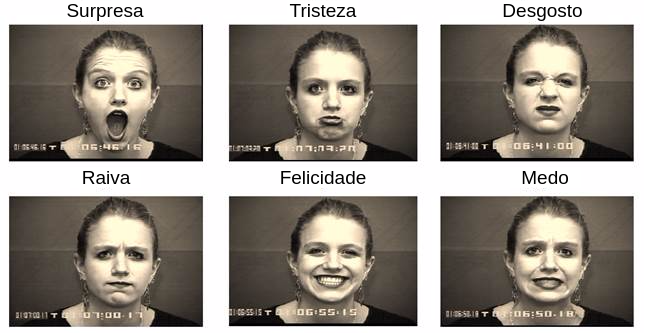
\includegraphics[scale=0.7]{figuras/facesbasicas.png}
\caption{Expressão facial emocional}
\label{fig:facesbasicas}
\end{figure}

\section{Aprendizagem de Máquina}\label{sec:apm}
Com intuito de criar sistemas que possuem a capacidade de reconhecer emoção de forma automática é muito comum o emprego de técnicas de aprendizagem de máquina, que é um ramo da inteligência artificial em que máquinas aprendem a partir de uma experiência e são habilitadas para reconhecer padrões. Uma definição de aprendizagem de máquina foi dada por \cite{alpaydin2014introduction}: \emph{“É a programação de computadores para otimizar um critério de desempenho usando dados de exemplo ou experiência passada”}. Na prática, isto pode ser entendido como a existência de um modelo definido com alguns parâmetros, no qual a ação de aprender consiste na execução de uma função de otimização, cujos parâmetros do modelo são otimizados, a partir dos dados de treinamento ou experiência passada. O modelo pode ser preditivo, para fazer previsões do futuro; descritivo, para obter conhecimento dos dados realizando a classificação; ou ambos.

Em aprendizagem de máquina, se as instâncias são conhecidas, isto é,  cada  instância possui o seu rótulo, então o aprendizado é supervisionado.  Caso contrário, se as instâncias são desconhecidas, a aprendizagem é não supervisionada. Neste trabalho, o aprendizado utilizado é o supervisionado no qual os métodos possuem uma fase de treinamento e outra de teste. A primeira consiste na utilização de um conjunto de características com instâncias previamente rotuladas, também conhecido como base de treino, com objetivo de encontrar padrões nos exemplos e, assim, produzir um modelo para armazenar o aprendizado. Por fim, na fase de teste, o algoritmo deve classificar dados desconhecidos, por meio da base de teste, a partir dos padrões encontrados na fase anterior e mensurar o desempenho obtido. Além disso, o modelo gerado pode ser testado por outra base chamada de validação para averiguar com mais confiança que não há aprendizagem viciosa. Caso o desempenho esteja satisfatório o método está apto para a produção, senão deve voltar para fase de treinamento \citep{kotsiantis2007supervised, geron2017hands}.

\section{Processo de Classificação de Imagem}\label{sec:pci}
Nos problemas de classificação de imagem, quando a abordagem é por meio da aprendizagem de máquina, geralmente é seguido o processo: (i) a etapa inicial consiste em uma fase de pré-processamento em que são aplicadas várias técnicas com a intenção de eliminar o ruído da imagem, resultando em sua melhora considerável para as fases posteriores; (ii) a etapa de extração de característica foca em destacar ou retirar as principais formas da imagem que são importantes para a separação das classes e (iii) as características extraídas são enviadas para um classificador determinar qual a classe que a imagem pertence.

\section{Técnicas para pré-processamento de imagens em reconhecimento de emoção por expressão facial}\label{sec:tecnic}
\subsection{Detecção Facial}\label{sec:detecfacialviola}
Este procedimento consiste na utilização de técnicas que verificam a existência de uma face em uma imagem, seja em uma fotografia ou \textit{frame} de vídeo. Geralmente é um problema difícil, pois dado uma imagem o método deve detectar em qual região há faces. No entanto, uma imagem pode ter diferentes objetos, \textit{backgrounds} e ruídos. A união desses elementos pode induzir o método a identificar erroneamente uma face, causando confusão e a ocorrência de falsos positivos, isto é, objetos sendo incorretamente identificados como face.

\begin{figure}
\centering
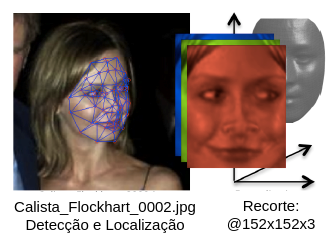
\includegraphics[scale=0.75]{figuras/detectface.png}
\caption{Detecção Facial}
\label{fig:detectface}
\end{figure}


O algoritmo Viola-Jones \citep{viola2001rapid} é amplamente usado pela comunidade para detecção facial. Esta técnica possui vantagens como alta taxa de precisão, rapidez na execução e baixa taxa de falsos positivos. Este algoritmo é utilizado por \cite{art1}, \cite{art2}, \cite{art6}, \cite{art9}, \cite{art12}, \cite{art13} e \cite{art15} para detectar a face em uma imagem e realizar o recorte com o intuito de excluir o \textit{background} da imagem, reduzindo assim a complexidade do problema e diminuindo a carga de aprendizado da rede na qual, neste caso, o classificador não necessita mais aprender a diferenciar o que é \textit{background} e face.

\subsection{Histograma de Equalização (Normalização do Brilho)}
A técnica de histograma de equalização é utilizada para normalizar o brilho da imagem \citep{jain1989fundamentals}. Obviamente há diferentes tipos de ambiente e consequentemente a iluminação pode variar bastante. Esta técnica permite que a intensidade das cores seja melhor distribuída. A atuação desta técnica equilibra o contraste da imagem nas regiões em que há ausência.

Esta técnica foi utilizada por \cite{art2}, \cite{art4} e \cite{art6}. Para todos os casos resultou no aumento da taxa de acurácia comparada a não aplicação desta técnica. Provavelmente o histograma de equalização funciona principalmente porque busca equalizar as cores da imagem retirando os ruídos de iluminação, isto é, realçando todos os pontos da imagem ocasionando maior facilidade para aprendizagem do problema devido a maximização da visibilidade nas regiões importantes que separam as classes, além disso, há a diminuição da carga de aprendizado do classificador, pois é menos necessário aprender a separar as classes nos casos de iluminação adversa.

%realçando todos os pontos da imagem ocasionando maior visibilidade das regiões importantes e o método de classificação aprende com maior facilidade a separar as classes, além disso, há a diminuição da carga de aprendizado, pois é menos necessário aprender a separar as classes nos casos de iluminação adversa.

%o primeiro por reduzir a carga de aprendizado da rede, pois nas situações em que uma imagem não possui a iluminação ideal a rede não precisa aprender essas situações adversas;

\section{Rede Neural Artificial}\label{sec:rna}
O ser humano inspirou-se nos pássaros para construir aeronaves e voar. A natureza também inspirou outras invenções da humanidade, por exemplo a dianteira de um trem-bala. Da mesma forma, as redes neurais artificiais tiveram a mesma inspiração, especificamente no cérebro, tendo como objetivo construir máquinas inteligentes \citep{geron2017hands, goodfellow2016deep}. 

Um \textit{perceptron}, que é uma simples arquitetura inspirada em um neurônio biológico, possui conexões de entrada e saída para conectar a outros neurônios. Cada conexão de entrada é associada a um peso, que recebe um sinal para o neurônio realizar uma computação baseada em uma função de ativação, gerando um sinal de saída que serve de entrada para outro neurônio \citep{geron2017hands}. 

A Figura \ref{fig:redeneural} ilustra uma rede neural \textit{perceptron} multicamadas.  A rede neural \textit{perceptron} possui uma estrutura em que consiste de uma camada de entrada, várias camadas intermediárias denominadas ocultas e uma camada de saída. Todas as camadas são compostas por neurônios \textit{perceptron}. A camada de entrada recebe os dados oriundos de uma instância, por exemplo, os \textit{pixels} de uma imagem, e encaminha os dados recebidos para a próxima camada. A camada oculta caracteriza-se por ser completamente conectada, isto é, cada neurônio conecta-se com todos da camada anterior e posterior. A camada de saída é responsável em fornecer o resultado da rede neural, por isso, nos casos de classificação, a quantidade de neurônio da camada de saída é a mesma das classes do problema. Além disso, cada neurônio da camada de saída está associada a uma classe e quando uma instância desconhecida for processada para classificação, o neurônio que terminar ativado da camada de saída representa a classificação desta instância \citep{geron2017hands, goodfellow2016deep}.

\begin{figure}
\centering
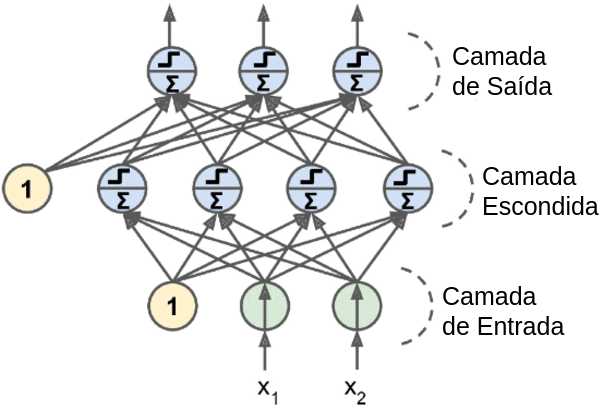
\includegraphics[scale=0.45]{figuras/redeneural.png}
\caption{Rede Neural Artificial}
\label{fig:redeneural}
\end{figure}

\section{Rede Neural de Convolução}\label{sec:rnc}
As redes neurais de convolução (RNC) surgiram dos estudos do córtex visual do cérebro e têm sido usadas em reconhecimento de imagem desde 1980 \citep{geron2017hands}. Nos últimos anos, uma série de fatores contribuíram para a evolução das RNCs, principalmente relacionados ao aumento do poder de computação (hardware), ao surgimento da web, que proporcionou o aumento da quantidade de dados para treinamento e à evolução das técnicas de treinamento de uma rede neural. Este cenário favorável permitiu que as RNCs alcançassem nível super-humano em alguns problemas complexos de visão computacional. As RNCs têm sido utilizadas em larga escala tanto pela indústria como pelos pesquisadores, sobretudo em problemas como máquinas de busca, carros autônomos, sistemas de classificação automática de vídeo e imagens, entre outras tarefas.


Os trabalhos de \cite{hubel1959single} e \cite{hubel1959receptive} realizaram uma série de experimentos em gatos em 1958, e posteriormente, em macacos \citep{hubel1968receptive}, para encontrar intuições do funcionamento do córtex visual, que é a parte cerebral responsável em processar informação visual. Estes trabalhos levaram os autores a receberem o Prêmio Nobel em Fisiologia e Medicina em 1981. Seus trabalhos mostraram que muitos neurônios do córtex visual tem um pequeno campo de recepção local, ou seja, os neurônios reagem somente a um estímulo localizado na região limitada pelo campo visual. O campo de recepção local dos diferentes neurônios podem sobrepor um ao outro e a sua combinação gera o campo visual. Os autores mostraram que alguns neurônios somente reagem às imagens com padrões de linhas horizontais enquanto outros reagem às linhas com diferentes orientações. Notou-se que alguns neurônios têm um campo grande de recepção local, consequentemente, reagindo aos padrões mais complexos. Entretanto, os neurônios estão combinando um ao outro para gerar padrões menos complexos. Estas observações são evidências de que os neurônios são baseados na saída do vizinho. 

O poderoso funcionamento do córtex visual está habilitado a detectar todos os padrões complexos em qualquer área do campo visual \citep{geron2017hands}. Todos os estudos relacionados ao córtex visual foram gradualmente inseridos nas redes neurais artificiais para gerar a rede neural de convolução. A primeira RNC  foi apresentada por \cite{lecun1998gradient}, uma arquitetura denominada LeNet-5 que foi utilizada para reconhecer dígitos escritos no papel.

\subsection{Camada de Convolução}
A camada de convolução é o mais importante bloco de uma RNC e consiste em uma operação matemática que desliza uma função sobre a outra calculando a integral entre a multiplicação de duas funções. A Figura \ref{fig:conv1} ilustra o que cada camada de convolução recebe em seu campo visual dada uma imagem como entrada na RNC. Vale ressaltar que cada neurônio da primeira camada de convolução está conectado somente a alguns campos visuais de recepção da imagem, diferentemente da abordagem tradicional que é conectada a todos os \textit{pixels}. Os neurônios da segunda camada de convolução estão conectados somente aos localizados no pequeno campo visual (retângulo) da primeira camada, novamente diferente da rede neural \textit{perceptron} em que todos os neurônios são conectados com todos da camada anterior, e assim por diante \citep{geron2017hands}. As vantagens da RNC sobre a abordagem tradicional são explicadas pela diferença entre ambas e são enfatizadas a seguir:

\begin{enumerate}[label=(\roman*)]
 \item A RNC tem característica esparsa como ilustrado na Figura \ref{fig:conv2}, por isso, a RNC possui menor quantidade de parâmetros para serem treinados do que as redes neurais tradicionais, isto é, requer menos tempo de treinamento e recursos computacionais \citep{goodfellow2016deep}; 
\item A estrutura da RNC é comum no mundo real, por exemplo no córtex visual. Essa inspiração biológica é uma das razões para RNC funcionar tão bem no reconhecimento de imagens \citep{geron2017hands}; 
\item E por fim, o compartilhamento de parâmetros resulta no aprendizado de rotações dos objetos da imagem e os neurônios aprendem em conjunto ao invés de separados \citep{goodfellow2016deep}.
\end{enumerate}


\begin{figure}
\centering
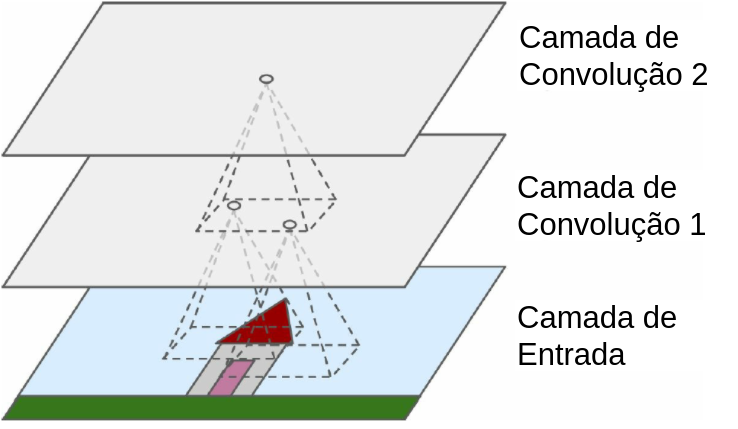
\includegraphics[scale=0.40]{figuras/conv1.png}
\caption{Camada de Convolução com campos locais de recepção}
\label{fig:conv1}
\end{figure}

\begin{figure}
\centering
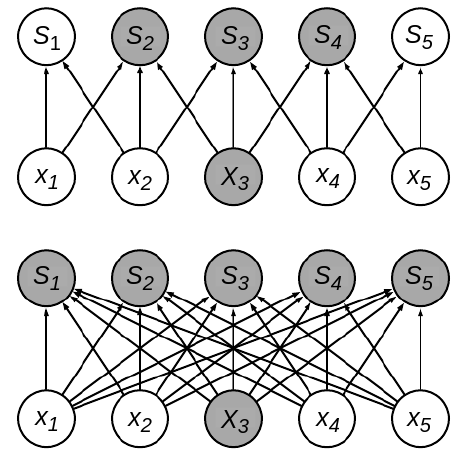
\includegraphics[scale=0.6]{figuras/conv2.png}
\caption{Conectividade esparsa. É destacada a entrada \textit{x}\textsubscript{3} e a saída em S que são afetadas por \textit{x}\textsubscript{3}. 
(Cima) Quando S recebe a convolução com um \textit{kernel} de tamanho 3, somente três saídas são afetadas por \textit{x}\textsubscript{3}. 
(Baixo) Quando S é gerado por rede neural tradicional, todos são afetados por \textit{x}\textsubscript{3}.}

%\caption{Conectividade esparsa. É destacada a entrada x\textsubscript{3} e a saída em S que são afetadas por x\textsubscript{3}}
\label{fig:conv2}
\end{figure}


\subsection{Camada de \textit{Pooling}}
Esta camada tem como foco principal realizar subamostra, isto é, diminuir o tamanho de entrada da imagem entre as camadas de convolução com objetivo de reduzir a carga computacional e o número de parâmetros, ocasionando a diminuição do risco de \textit{overfitting} e o consumo de memória \citep{geron2017hands}. Além disso, reduzir o tamanho de entrada da imagem faz a rede neural mais tolerável a variação do objeto principal, como a rotação da face. 

Geralmente uma camada de \textit{pooling} é implementada logo após uma camada de convolução, portanto recebe como entrada uma imagem processada anteriormente por uma camada de convolução com intuito de realizar subamostra da imagem e encaminhar o resultado para uma próxima camada de convolução \citep{goodfellow2016deep}.

Existem duas principais funções de \textit{pooling}. Por exemplo, o \textit{max pooling} que considera o valor máximo de um campo de recepção e está exemplificado na Figura \ref{fig:pool} por um \textit{kernel} 2x2 que elimina 75\% dos valores de entrada. Há também o \textit{pooling} pela média de um campo de recepção e seu cálculo consiste na distância entre o \textit{pixel} central e seus vizinhos \citep{goodfellow2016deep}. A camada de \textit{max pooling} é a mais comum operação de \textit{pooling} utilizada em redes neurais de convolução.


\begin{figure}
\centering
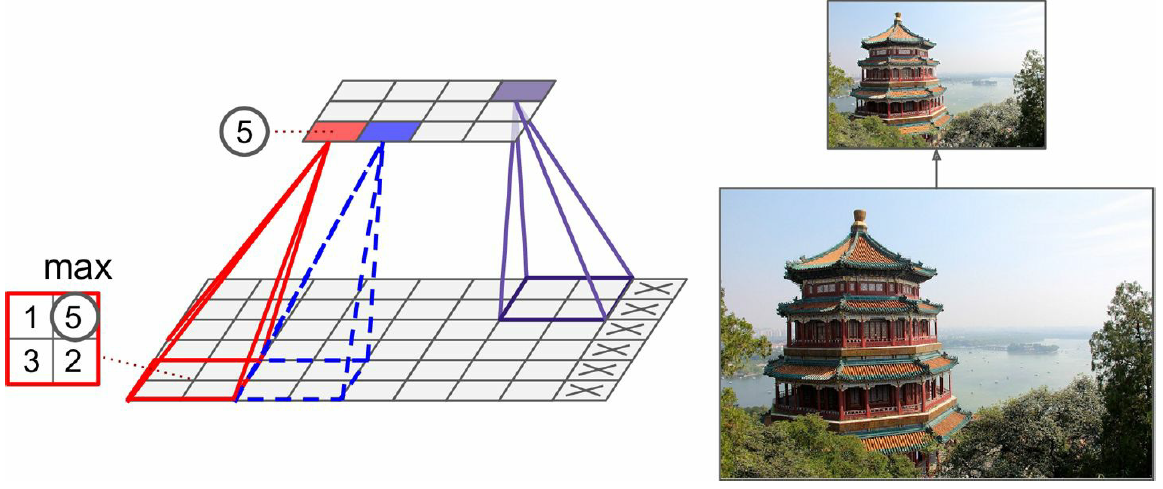
\includegraphics[scale=0.45]{figuras/pool.png}
\caption{Camada de \textit{Max Pooling}}
\label{fig:pool}
\end{figure}


\subsection{Regressão \textit{Softmax}}
Geralmente uma arquitetura de RNC é composta em sua maior parte por camadas de convolução e \textit{pooling}. Estas camadas processam a imagem com intuito de extrair os principais padrões para um classificador e determinar a classe dela. Por isso, ao final de uma arquitetura de RNC é necessário um classificador que tradicionalmente tem sido o \textit{softmax}. Este classificador é um modelo generalizado de uma regressão logística, que por sua vez é normalmente usada para estimar probabilidades de uma instância pertencer a uma classe em particular, por exemplo, qual é a probabilidade de um email ser spam? \citep{geron2017hands}. Se a estimativa de probabilidade for maior que 50\%, então o modelo prevê que a instância pertence a classe positiva, caso contrário, pertence à classe negativa. Portanto, isto faz do regressor logístico um classificador binário. Um \textit{softmax} é capaz de estimar probabilidades para múltiplas classes e não há a necessidade de treinar e combinar múltiplos classificadores binários para tal tarefa. Um \textit{softmax} está habilitado a estimar probabilidades para uma imagem processada em uma RNC e, para todos os efeitos, a imagem é uma expressão facial que pertence às emoções básicas: neutralidade, felicidade, surpresa, medo, raiva, tristeza ou desgosto.

\section{Arquiteturas de Redes Neurais de Convolução}\label{sec:arc}
\subsection{AlexNet}

A arquitetura AlexNet foi desenvolvida por Alex Krizhevsky (por isso, o nome da mesma), Ilya Sutskever e Geoffrey Hinton. Destacando-se por ser grande e muito profunda, a AlexNet foi a primeira RNC a empilhar camadas de convolução diretamente em cima da outra, ao invés da tradicional conexão entre uma camada de convolução e a camada de \textit{pooling}. Esta arquitetura pode ser consultada na Tabela \ref{alexnet}.

A AlexNet usa uma normalização bastante eficiente entre as camadas C1 e C3 denominada \textit{local response normalization}. Essa forma de normalização causa um efeito que contribui para inibição dos neurônios em ativar mais fortemente no mesmo local, ocasionando que outros mapas de características se tornem também especialistas em determinada região da imagem. Este comportamento também é observado nos neurônios biológicos \citep{geron2017hands}. 

O seu grande sucesso foi devido ao desafio de 2012 do ImageNet ILSVRC, que tem sido o principal concurso de classificação de imagens organizado pela comunidade científica, em que venceu por uma margem bastante grande: alcançou 17\% no top-5 da taxa de erro, enquanto o segundo melhor alcançou somente 26\%!

\begin{table}[]
\caption{Arquitetura AlexNet}
\centering
\begin{tabular}{|c|c|c|c|c|c|}
\hline
\textbf{Camada} & \textbf{Tipo}           & \textbf{Mapas} & \textbf{Tamanho} & \textbf{Kernel} & \textbf{Ativação} \\ \hline
Saída           & Completamente Conectada & -              & 1000             & -               & Softmax           \\ \hline
F9              & Completamente Conectada & -              & 4096             & -               & ReLU              \\ \hline
F8              & Completamente Conectada & -              & 4096             & -               & ReLU              \\ \hline
C7              & Convolução              & 256            & 13 x 13          & 3 x 3           & ReLU              \\ \hline
C6              & Convolução              & 384            & 13 x 13          & 3 x 3           & ReLU              \\ \hline
C5              & Convolução              & 384            & 13 x 13          & 3 x 3           & ReLU              \\ \hline
S4              & \textit{Max Pooling}    & 256            & 13 x 13          & 3 x 3           & -                 \\ \hline
C3              & Convolução              & 256            & 27 x 27          & 5 x 5           & ReLU              \\ \hline
S2              & \textit{Max Pooling}    & 96             & 27 x 27          & 3 x 3           & -                 \\ \hline
C1              & Convolução              & 96             & 55 x 55          & 11 x 11         & ReLU              \\ \hline
Entrada         & Entrada                 & 3 (RGB)        & 224 x 224        & -               & -                 \\ \hline
\end{tabular}
%\caption{AlexNet arquitetura}
%\label{my-label}
\label{alexnet}
\end{table}


\subsection{GoogLeNet}

A arquitetura GoogLeNet \citep{szegedy2015going} foi desenvolvida por Christian Szegedy do \textit{Google Research}, e venceu o desafio do ILSVRC 2014 por alcançar a taxa de erro no top-5 abaixo de 7\%. Este grande desempenho foi devido em grande parte pelo fato de que a rede foi muito mais profunda do que as anteriores. O aumento de profundidade está diretamente relacionado à criação de sub-redes chamadas de \textit{inception} e está ilustrada na Figura \ref{fig:inception}. Essas sub-redes permitiram que a GoogLeNet utilizasse os parâmetros de forma mais eficiente comparada às arquiteturas anteriores e a dimensão desta eficiência pode ser elucidada pela diferença de parâmetros entre a GoogLeNet e a AlexNet, em que a primeira possui 10 vezes menos parâmetros do que a segunda \citep{geron2017hands}. 

Um módulo \textit{inception}, que está ilustrado na Figura \ref{fig:inception}, possui uma notação ''3 x 3 + 2 (S)''. Isto significa que a camada usa um \textit{kernel} 3 x 3, \textit{stride} 2 e \textit{SAME padding}. O sinal de entrada é primeiramente copiado e alimenta as camadas do módulo \textit{inception} que estão divididas em dois conjuntos. O primeiro conjunto recebe o sinal para processar e encaminhar para o segundo. Vale ressaltar que todas as camadas de convolução utilizam a ReLU como função de ativação. É interessante observar que o segundo conjunto usa diferentes tamanhos de \textit{kernel} (1 x 1, 3 x 3 e 5 x 5), permitindo que a rede possa capturar diferentes padrões de escala \citep{geron2017hands}. No fim do módulo, há uma camada de concatenação, isto é, combina todas as saídas do segundo conjunto de camadas de convolução e encaminha um único sinal que é o resultado do módulo para uma próxima camada da rede. A rede GoogLeNet é composta por módulos \textit{inception}, camadas de convolução, \textit{max pooling}, camadas de \textit{local normalization response}, camadas completamente conectadas e \textit{softmax}.


\begin{figure}
\centering
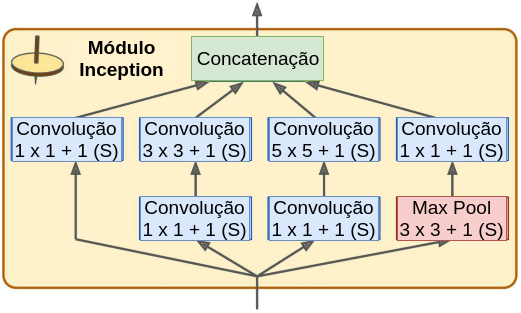
\includegraphics[scale=0.6]{figuras/inception.png}
\caption{Módulo \textit{inception}}
\label{fig:inception}
\end{figure}


\subsection{VGGNet}
Proposta por \cite{simonyan2014very}, a VGGNet foi a vice-campeã do desafio ILSVRC 2014, tendo alcançado 6.8\% na taxa de erro top-5. A sua principal contribuição foi uma avaliação exaustiva de seis RNCs, que consistiu no aumento de profundidade enfatizando a utilização de filtros de convolução com tamanho muito pequeno (3 x 3), promovendo o aumento da profundidade da rede que passou de 16 para 19 camadas. Esta abordagem mostrou um aumento de eficiência significativo comparado às técnicas anteriores. 

A VGGNet é composta principalmente por camadas de convolução, \textit{max pooling}, completamente conectadas e \textit{softmax}, e está ilustrada na Tabela \ref{tab:vgg}. O fato de usar filtros de convolução com tamanho pequeno ocasionou no não aumento do número de parâmetros a serem ajustados a medida que a rede cresce, promovendo assim a eficiência.

%\begin{figure}
%\centering
%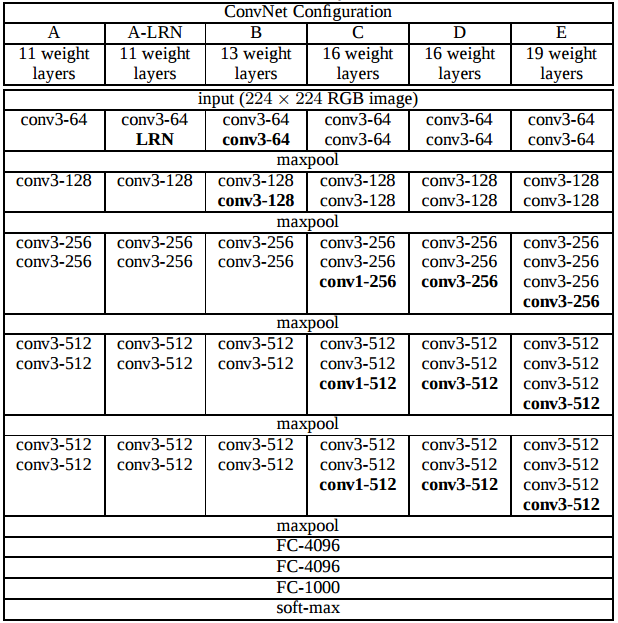
\includegraphics[scale=0.6]{figuras/vgg.png}
%\caption{VGGNet}
%\label{fig:vgg}
%\end{figure}


\begin{table}[]
\centering
\caption{Arquiteturas VGGNet}
\label{tab:vgg}
\begin{tabular}{|c|c|c|c|c|c|}
\hline
\multicolumn{6}{|c|}{\textbf{VGGNet configuração}}                                                                                                                                                                                                                                                                                                                                                                                               \\ \hline
A                                                             & A-LRN                                                         & B                                                             & C                                                                         & D                                                                         & E                                                                                     \\ \hline
11 camadas                                                    & 11 camadas                                                    & 13 camadas                                                    & 16 camadas                                                                & 16 camadas                                                                & 19 camadas                                                                            \\ \hline
\multicolumn{6}{|c|}{camada de entrada (224 x 224 imagem RGB)}                                                                                                                                                                                                                                                                                                                                                                                \\ \hline
conv3-64                                                      & \begin{tabular}[c]{@{}c@{}}conv3-64\\ \textbf{LRN}\end{tabular}        & \begin{tabular}[c]{@{}c@{}}conv3-64\\ \textbf{conv3-64}\end{tabular}   & \begin{tabular}[c]{@{}c@{}}conv3-64\\ conv3-64\end{tabular}               & \begin{tabular}[c]{@{}c@{}}conv3-64\\ conv3-64\end{tabular}               & \begin{tabular}[c]{@{}c@{}}conv3-64\\ conv3-64\end{tabular}                           \\ \hline
\multicolumn{6}{|c|}{maxpool}                                                                                                                                                                                                                                                                                                                                                                                                                 \\ \hline
conv3-128                                                     & conv3-128                                                     & \begin{tabular}[c]{@{}c@{}}conv3-128\\ \textbf{conv3-128}\end{tabular} & \begin{tabular}[c]{@{}c@{}}conv3-128\\ conv3-128\end{tabular}             & \begin{tabular}[c]{@{}c@{}}conv3-128\\ conv3-128\end{tabular}             & \begin{tabular}[c]{@{}c@{}}conv3-128\\ conv3-128\end{tabular}                         \\ \hline
\multicolumn{6}{|c|}{maxpool}                                                                                                                                                                                                                                                                                                                                                                                                                 \\ \hline
\begin{tabular}[c]{@{}c@{}}conv3-256\\ conv3-256\end{tabular} & \begin{tabular}[c]{@{}c@{}}conv3-256\\ conv3-256\end{tabular} & \begin{tabular}[c]{@{}c@{}}conv3-256\\ conv3-256\end{tabular} & \begin{tabular}[c]{@{}c@{}}conv3-256\\ conv3-256\\ \textbf{conv1-256}\end{tabular} & \begin{tabular}[c]{@{}c@{}}conv3-256\\ conv3-256\\ \textbf{conv3-256}\end{tabular} & \begin{tabular}[c]{@{}c@{}}conv3-256\\ conv3-256\\ conv3-256\\ \textbf{conv3-256}\end{tabular} \\ \hline
\multicolumn{6}{|c|}{maxpool}                                                                                                                                                                                                                                                                                                                                                                                                                 \\ \hline
\begin{tabular}[c]{@{}c@{}}conv3-512\\ conv3-512\end{tabular} & \begin{tabular}[c]{@{}c@{}}conv3-512\\ conv3-512\end{tabular} & \begin{tabular}[c]{@{}c@{}}conv3-512\\ conv3-512\end{tabular} & \begin{tabular}[c]{@{}c@{}}conv3-512\\ conv3-512\\ \textbf{conv1-512}\end{tabular} & \begin{tabular}[c]{@{}c@{}}conv3-512\\ conv3-512\\ \textbf{conv3-512}\end{tabular} & \begin{tabular}[c]{@{}c@{}}conv3-512\\ conv3-512\\ conv3-512\\ \textbf{conv3-512}\end{tabular} \\ \hline
\multicolumn{6}{|c|}{maxpool}                                                                                                                                                                                                                                                                                                                                                                                                                 \\ \hline
\begin{tabular}[c]{@{}c@{}}conv3-512\\ conv3-512\end{tabular} & \begin{tabular}[c]{@{}c@{}}conv3-512\\ conv3-512\end{tabular} & \begin{tabular}[c]{@{}c@{}}conv3-512\\ conv3-512\end{tabular} & \begin{tabular}[c]{@{}c@{}}conv3-512\\ conv3-512\\ \textbf{conv1-512}\end{tabular} & \begin{tabular}[c]{@{}c@{}}conv3-512\\ conv3-512\\ \textbf{conv3-512}\end{tabular} & \begin{tabular}[c]{@{}c@{}}conv3-512\\ conv3-512\\ conv3-512\\ \textbf{conv3-512}\end{tabular} \\ \hline
\multicolumn{6}{|c|}{maxpool}                                                                                                                                                                                                                                                                                                                                                                                                                 \\ \hline
\multicolumn{6}{|c|}{camada completamente conectada - 4096}                                                                                                                                                                                                                                                                                                                                                                                   \\ \hline
\multicolumn{6}{|c|}{camada completamente conectada - 4096}                                                                                                                                                                                                                                                                                                                                                                                   \\ \hline
\multicolumn{6}{|c|}{camada completamente conectada - 1000}                                                                                                                                                                                                                                                                                                                                                                                   \\ \hline
\multicolumn{6}{|c|}{softmax}                                                                                                                                                                                                                                                                                                                                                                                                                 \\ \hline
\end{tabular}
\end{table}

\subsection{Residual Network}
A Residual Network (ou ResNet) foi desenvolvida por \cite{he2016deep} e foi a técnica vencedora do desafio ILSVRC 2015. A ResNet foi avaliada na base de teste do ImageNet que tinha 1000 classes e alcançou 3.6\% em taxa de erro no top-5, ou seja, quando uma imagem é classificada este tipo de avaliação consiste na verificação das 5 classes com maior probabilidade, e caso esta imagem pertencer ao grupo das 5 classes caracteriza-se uma classificação correta. A ResNet proposta para o concurso tinha 152 camadas caracterizando uma rede muito profunda. 

O segredo desta técnica consiste na composição dos blocos residuais. Tais blocos trazem novidades     


\subsection{\textit{Ensemble}}
Suponha uma questão complexa perguntada aleatoriamente para milhões de pessoas, então, todas as respostas são agregadas para obter o resultado. Em muitos casos, a resposta agregada é melhor do que a de um especialista. Isto é conhecido como sabedoria popular. Similarmente, se agregar as classificações de uma determinada instância oriunda de um grupo de RNCs e, frequentemente, tem mais acertos do que a classificação de uma única RNC. Um grupo de RNCs ou outros tipos de classificadores e regressores são chamados de \textit{ensemble} \citep{geron2017hands}. Geralmente, quem trabalha com \textit{ensemble} no problema de reconhecimento de emoção tem calculada a média das probabilidades estimadas pelas diversas RNCs para decidir qual a classificação final da expressão facial.

\section{Resumo}\label{sec:considf}
Neste capítulo foram apresentados os principais conceitos utilizados por esta proposta. Foi visto que uma RNC, que é uma técnica de aprendizagem de máquina, foi projetada para a classificação de imagem, justificando a sua escolha para a classificação de emoções em expressão facial. Esta técnica é muito poderosa e tem sido inspirada no cérebro dos mamíferos. A expressão facial tem se destacado como uma forma eficaz de coleta de dados para o reconhecimento de emoção, principalmente, por ser ubíqua, não intrusiva e pela popularidade de dispositivos que contém câmeras fotográficas. Entretanto, somente as emoções básicas são possíveis de reconhecer por meio da expressão facial. Isso significa que reconhecer tédio, frustração e confusão se torna bastante difícil por esse meio. Além disso, técnicas de pré-processamento, tais como histograma de equalização e detecção com recorte da face são úteis durante o processo de classificação de imagens, justamente por diminuir a carga de aprendizado da rede. Por fim, foram conceituadas algumas das principais arquiteturas de RNCs em que cada uma possui sua característica em particular que precisam ser experimentadas em diferentes cenários.  
